\section{The graphic and the exact cyclicity statement}
\label{sec:introduction}
The quadratic graphic $DF_{1b}$ consists of a fast arc and a segment
of equilibria ending at a nilpotent contact. Periodic orbits approaching
this entire graphic can have unbounded passage times as several unfolding
scales tend to zero. We prove that its whole-graphic cyclicity is exactly
two and obtain a common upper bound without restricting the relative
rates of the unfolding parameters.
Huzak explicitly excludes this contact endpoint from the results of
\cite[Remark~2, p.~1307]{Huzak2018} and identifies it as requiring
different techniques. We estimate its complete return through root
collision and simultaneous endpoint degeneration.

Consider the real quadratic family
\begin{equation}\label{eq:family}
 \dot z=y(1+bz-y)+\mu_1+\mu_2z+\mu_3z^2,\qquad
 \dot y=zy+\mu_4,\qquad 0<b<2,
\end{equation}
where $\mu=(\mu_1,\mu_2,\mu_3,\mu_4)$ is the raw unfolding parameter
and $b$ is a modulus. At $\mu=0$, division by $y$ in the positive
half-plane gives the fast system
\begin{equation}\label{eq:fast}
 z'=1+bz-y,\qquad y'=z.
\end{equation}
Let $\gamma_b$ be its positive-time orbit from $(0,0)$ to its first
subsequent intersection $(f_b,0)$ with the axis. Then $f_b<0$ and
\begin{equation}\label{eq:graphic}
 \Gamma_b=\Gamma_0^b:=\gamma_b\cup([f_b,0]\times\{0\})
\end{equation}
is a Jordan curve. The fast solution and the sections in Figure~\ref{fig:graphic}
are constructed in Appendix~\ref{sec:geometry}.
This is $DF_{1b}$ in the quadratic graphic classification.

Write $d_{\rm H}$ for two-sided Hausdorff distance. If $L$ is an isolated
periodic orbit, its multiplicity $m(L)$ is the order of the zero of
$P(s)-s$ for the actual finite minimal Poincar\'e return on a physical
analytic transverse section. Analytic changes between physical sections
preserve this order. The multiplicity will be one or two in the proof.

Throughout this paper cyclicity refers to convergence to the entire
graphic. More explicitly, for fixed $b$ set
\[
 C_{\rm H}(b)=\inf_{\eta>0}\
 \sup_{\|\mu\|<\eta}
 \#\{L:\ L\text{ is an isolated periodic orbit of }X_{b,\mu},
                         \ d_{\rm H}(L,\Gamma_b)<\eta\}.
\]
The whole-Hausdorff condition also places $L$ in any prescribed
phase neighborhood when $\eta$ is sufficiently small.
The stronger upper assertion below counts actual multiplicity.

\begin{samepage}
\begin{theorem}\label{thm:main}
For the family \eqref{eq:family} the following assertions hold.
\begin{enumerate}
\item For every compact interval $J\Subset(0,2)$ there are a common
compact phase neighborhood $K$ of $\bigcup_{b\in J}\Gamma_b$, an open
raw parameter neighborhood $V\subset\R^4$ of zero, and
$\rho_{\rm H}>0$ such that, for every $(b,\mu)\in J\times V$,
\begin{equation}\label{eq:upper-total}
 \sum_{\substack{L\ {\rm isolated}\\L\subset K,\
                         d_{\rm H}(L,\Gamma_b)<\rho_{\rm H}}}m(L)\le2 .
\end{equation}
\item For each fixed $b\in(0,2)$ there are positive sequences
$c_n,\varepsilon_n,\nu_n$ such that
\begin{equation}\label{eq:realizing-parameters}
 \mu_n=(\varepsilon_n^2c_n,-\varepsilon_n^2,
                          \varepsilon_n^2,-\nu_n)\longrightarrow0,
\end{equation}
and the same field $X_{b,\mu_n}$ has two distinct isolated positive
periodic orbits $L_n^-,L_n^+$ satisfying
\begin{equation}\label{eq:two-whole-limits}
 d_{\rm H}(L_n^-,\Gamma_b)\longrightarrow0,\qquad
 d_{\rm H}(L_n^+,\Gamma_b)\longrightarrow0.
\end{equation}
After deletion of finitely many terms, both orbits have multiplicity one;
$L_n^-$ is hyperbolic repelling and $L_n^+$ is hyperbolic attracting.
Thus $\Gamma_b$ has cyclicity exactly two for each fixed $b\in(0,2)$.
\end{enumerate}
\end{theorem}
\end{samepage}

The upper assertion permits arbitrary relative rates of the raw
parameters and is uniform on compact modulus intervals. The realizing
sequences are chosen for each fixed $b$, and their periods may increase.
The whole-graphic count differs from the count of all cycles contained
in a tube: a cycle shrinking to a point of $\Gamma_b$ is excluded by the
two-sided Hausdorff condition.

\begin{figure}[H]
\centering
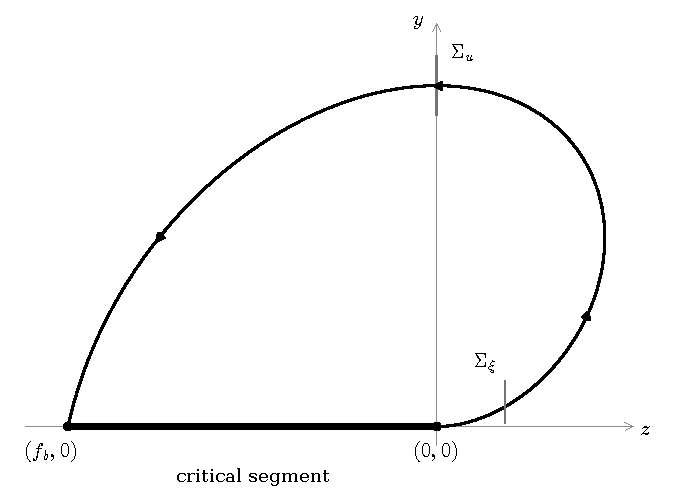
\includegraphics[width=.62\textwidth]{figures/df1b-graphic.pdf}
\caption{The graphic $\Gamma_0^b$ for $b=1/2$, plotted from
\eqref{eq:fast-orbit} with equal coordinate scales. The solid curve is
the fast arc; arrows indicate its direction. Every point of the thick
horizontal segment is an equilibrium of the unperturbed quadratic
field. The short vertical lines indicate transverse sections. The
graphic is not a periodic orbit.}
\label{fig:graphic}
\end{figure}


\subsection{Relation with earlier graphic problems}
The Dumortier--Roussarie--Rousseau program reduces the quadratic
limit-cycle problem to local cyclicity problems for a finite
classification of graphics \cite{DRR1994}. Theorem~\ref{thm:main} gives the sharp count for
cycles converging to this entire graphic. This is the Hausdorff notion
used in the actual counting
statements of \cite[Theorem~3.1]{DR2009} and
\cite[Theorems~1.1--1.2]{Huzak2018}.
The analytic affine and time normalization of
\cite[Proposition~2.1]{DR2009} identifies a neighborhood in the full
twelve-dimensional quadratic coefficient space with this family and
the coordinate and time changes. Using that known normalization,
Corollary~\ref{cor:quadratic-space} transfers the sharp whole-graphic
count to the full coefficient space: the total actual multiplicity is
at most two, and two simultaneous whole-graphic orbits realize the
bound. Corollary~\ref{cor:open-quadratic-realization} further gives
nonempty open sets of coefficients approaching each fixed base field,
with one attracting and one repelling cycle converging to the graphic.
\footnote{The numbering for
\cite{DR2009} refers to the November 30, 2007 author version,
\url{https://www.dms.umontreal.ca/~rousseac/Dumortier_Rousseau.pdf}.}

For normal slow--fast double-saddle cycles,
\cite[Theorem~2.25(ii)]{DMD2008Singular} gives an upper bound two. That result assumes
two persistent hyperbolic corners, a common slow scale with distinct
scaled characteristic ratios, and strict passage conditions between
the corners; Lemma~4.11 there retains the
signed splitting in the connection. Theorem~2.23 of the same paper
also treats certain interior slow saddle-node passages. In the present graphic the
right corner is the turning point itself. As a positive saddle
approaches that point, its characteristic ratio, the physical source
coordinate, and the connection scales degenerate together. Applying
a normal double-saddle comparison in this limit requires uniform
bounds for the complete composed return, including its source
derivatives and signed splitting.

For generic balanced multilayer canards with every side comparison
side-preserving,
\cite[Theorem~4.10, pp.~1346--1347]{DR2008Multilayer} models the actual
rescaled return by translated-power compositions with a controlled
remainder on compact subsets of their positive domain; Corollary~4.11
gives finite cyclicity bounds in that setting. The all-side-preserving
restriction is clarified in \cite{DMD2023SideComparison}.
The separate corrigendum
\cite[p.~1995]{DR2008Corrigendum} gives the smooth functions in equation~(8)
full layer-variable dependence; their single-variable dependence holds
only for their infinite jets at the layer origin.

For ordinary non-transitory canards crossing two open fast layers,
De Maesschalck, Dumortier and Roussarie treat all five connection
diagrams, including side-reversing connections \cite{DMR2025TwoLayer}.
Their Theorem~2 (p.~25), with Definitions~9--10 (p.~24), gives the bound
$\operatorname{Cod}(X)+1$, counting multiplicity, for any unfolding of a
special finite codimensional system $X$.
On its fixed compact layer rectangle, the bound holds for all parameters
in a common neighborhood and all $0<\varepsilon\le\varepsilon_0$, with
no restriction on their relative rates
\cite[proof of Theorem~2, Claim, p.~27]{DMR2025TwoLayer}.
Obtaining an upper bound two from this theorem requires a corresponding
model with $\operatorname{Cod}(X)\le1$.
The original $\Gamma_b$ has only an attracting slow segment and a fast
arc issuing from the contact, so it is not itself an ordinary two-layer
canard. The estimates below follow the signed physical connector
through the degenerating parameter windows, retaining its negative
offset, actual returning domain, and weighted derivatives.

The local contact results of \cite{DMD2010,DMD2011Detectable} provide
finite-order transition and scaled-divergence estimates for finite-order
singular slow dynamics. The global count in
\cite[Theorem~2.7]{DMD2011Detectable} uses normal entry and exit
corners, while Theorems~3.1--3.2 exclude simultaneous zeros of the
slow dynamics at both corners. For the quadratic graphics
$\Gamma_x^b$ whose fast orbit starts at $(x,0)$, the applications in
\cite[Theorem~7]{DMD2010} and
\cite[Theorems~1.1--1.2]{Huzak2018} take $x$ in a compact subset
of $(0,\infty)$. Their source parametrization is regular in that
domain. In the $b=0$ case of \cite{Huzak2018}, for example, the
upper-section height is $1+\sqrt{1+x^2}$, whose derivative vanishes
at $x=0$. We use a regular physical section on the fast arc of
$\Gamma_b$ and estimate the return at this contact endpoint directly.

\enlargethispage{2pt}
Exact smooth normal linearization for specific skew products whose
center dynamics is independent of the normal variables is proved in
\cite[Theorems~1.1 and~1.3, pp.~41--42]{DR2010Normal}; the one-center
result preserves a multiple zero at every parameter value.
Exact finite-smooth normal linearization is also available in
\cite[Theorem~3]{BDMD2011Normal} for a skew product with a fixed
normal spectral gap and sufficiently small center spectrum.\footnote{For \cite{BDMD2011Normal}, this is
Theorem~3, p.~4, of the October 1, 2010 author version; the published
article is cited in the bibliography.}
Our phase and amplitude constructions retain the selected invariant
graph, a common tube with finite phase-derivative bounds, the small
coupling factor in the coordinate shear, and the derivatives after
passage to physical sections
(Lemma~\ref{lem:uniform-normal-product}). These quantitative outputs
are used in the subsequent return comparisons.

\subsection{The counting mechanisms and the proof}
Two coupled degenerations determine the upper proof. At a collision
of slow roots, a through-passage can magnify the incoming height by
an unbounded factor. We retain that factor and cancel it in a weighted
derivative identity. The resulting size and logarithmic-curvature
bounds force one derivative ratio to cross its critical value in one
direction on the actual returning interval
(Lemma~\ref{lem:pc-ratio}). For negative forcing, the preceding slow
segment places every counted return in a common small source interval
before the collision. The through-passage and fiber-exit descriptions
there satisfy the same strict bounds across their finite junction
(Lemma~\ref{lem:pc-event-gluing}). This gives one bound for the field
across the collision.

When both endpoints degenerate, the intermediate map is
$H(a)=\Psi(\eta_0u(a)^R)$, where $\Psi(0)=-B_{\rm conn}<0$.
We retain the complete nonlinear connection. Its negative offset and
small positive derivative give $0<H<u^R$ on the returning interval;
a weighted second-derivative bound controls its contribution to the
return curvature. Source flatness makes the double-saddle comparison uniform both
for a small weak characteristic ratio and as that ratio approaches
one (Lemma~\ref{lem:flat-two-saddle-comparison}). The actual source
interval and the required weighted second-derivative bounds
are verified for this quadratic family. Once each parameter window
controls all counted cycles of one field, a finite cover of the raw
parameter directions gives the common upper bound.

For sharpness, the weak saddle passage is an exact power map with
exponent below one. Its complement is exponentially contracting on
a full signed source rectangle, including the unstable outlet
(Lemma~\ref{lem:realizing-complement}). A small negative splitting
produces a negative--positive--negative displacement on one actual
return interval. Its two zeros give two orbits of the same field;
the image bounds on the rectangle show that each orbit follows the
fast arc and the complete slow segment.

Sections~\ref{sec:return-framework}--\ref{sec:counting} fix the physical
return, normal-product coordinates and scalar comparisons.
Sections~\ref{sec:positive-constant} and~\ref{sec:two-endpoints}
verify the complete collision and connector estimates, and
Section~\ref{sec:parameter-cover} gives their common parameter cover.
The appendices supply the geometric and local passage estimates.
Section~\ref{sec:lower-main} realizes two whole-graphic orbits using
the full complement proved in Appendix~\ref{sec:lower-complement};
Section~\ref{sec:combination} obtains hyperbolicity from the multiplicity
bound. Section~\ref{sec:quadratic-transfer} transfers the result to the
full quadratic coefficient space.
The finite differentiability order in each coordinate argument is
fixed before the parameter windows are shrunk.
